\newpage


\section{Analisi}
\label{sec:analisi}
In questa sezione verrà effettuata un analisi sui risultati della simulazione, comparando il modello base con le estensioni effettuate ed infine con un modello allo stato dell´arte.

\subsection{Analisi Modello Base}
Qui verranno analizzati le percentuali di evacuati e di morti nel tempo al variare del numero di auto e pedoni per il modello base.
Come mostrato nel grafico \ref*{fig:analisi-base-evacuated}, i pedoni non presentano alcun 
cambiamento rilevante nel numero di evacuati al variare di diversi split, 
per le auto invece all'aumentare del numero di auto corrisponde un numero sempre minore di evacuati ed un tempo maggiore è richiesto.
Osservando le evacuazioni totali invece risulta che lo split migliore sia il 50\%-50\%, mentre lo split 0\%-100\% sia il peggiore.

Considerazioni simili possono essere fatte rispetto \ref*{fig:analisi-base-casualties} alle morti con bassisime variazioni per i pedoni,
mentre per le auto i casi peggiori risultano gli split 0\%-100\% e 25\%-75\%, mentre i casi restanti non comportano morti.
Infine le morti totali mostrano come lo split migliore con meno perdite sia 50\%-50\%, mentre il peggiore 0\%-100\%.

Analizzando la distribuzione della percentuale di evacuati nel tempo è possibile notare quanto tempo sia necessario per evacuare.
Si può osservare da \ref*{fig:analisi-base-evtimes} come all´aumentare del numero di auto la media tenda a spostarsi verso sinistra
in particolare nel caso 50\%-50\% due picchi sembrano formarsi un molto probabilmente
per le auto il primo mentre il secondo per i pedoni, quest´ultimo tende ad appiattirsi con il crescere del numero di auto fino a sparire nel caso 0\%-100\%.

\begin{figure}[ht]
    \centering
    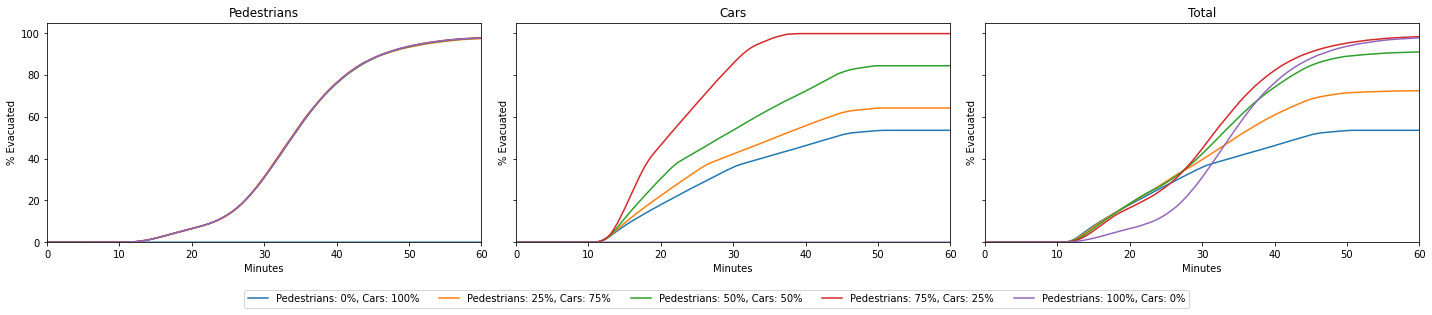
\includegraphics[width=\textwidth]{images/analisi/base-evacuated.png}
    \caption{percentuale pedoni e auto evacuati nel tempo per diversi split}
    \label{fig:analisi-base-evacuated}
\end{figure}

\newpage
\begin{figure}[ht]
    \centering
    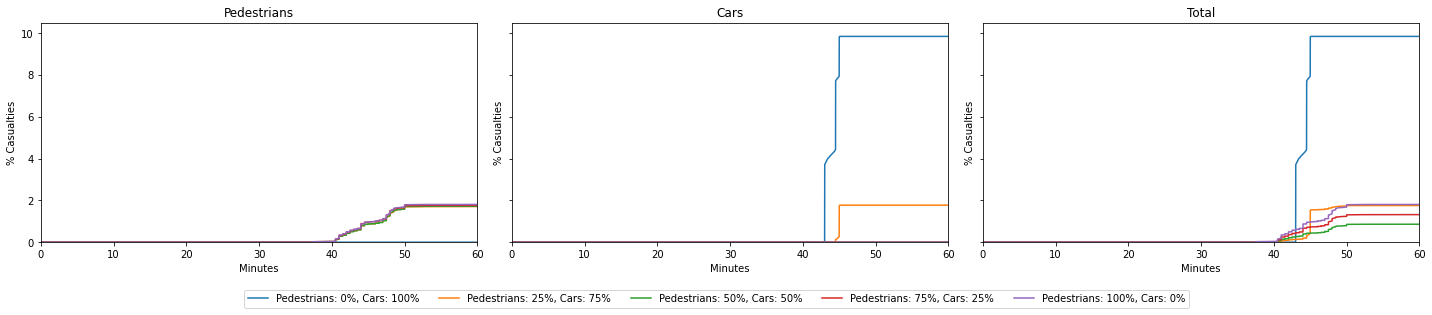
\includegraphics[width=0.8\textwidth]{images/analisi/base-casualties.png}
    \caption{percentuale pedoni e auto morti nel tempo per diversi split}
    \label{fig:analisi-base-casualties}
\end{figure}
%
\begin{figure}[ht]
    \centering
    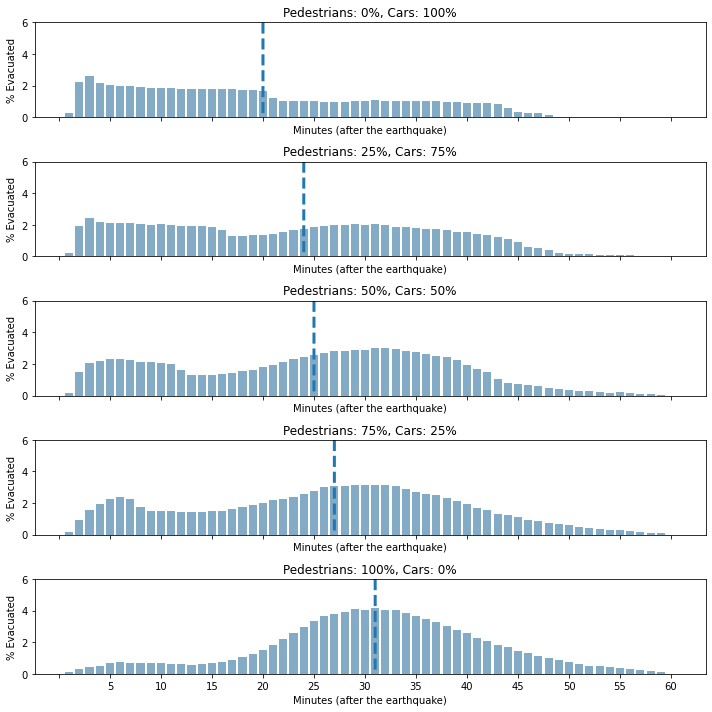
\includegraphics[width=0.8\textwidth]{images/analisi/base-evtimes.png}
    \caption{distribuzione nel tempo di evacuati in percentuale per diversi split}
    \label{fig:analisi-base-evtimes}
\end{figure}

\newpage

\subsection{Analisi Estensione Modello}
Le stesse analisi prese in considerazione per il modello base verranno descritte per il modello esteso.
Come mostrato nel grafico \ref*{fig:analisi-new-evacuated} andamento simile a quello visto in precedenza per il modello base
poche variazioni per i pedoni nella percentuale di evacuati leggermente più basa la curva corrispondente al caso 100\%-0\% probabilmente dovuta
ai rallentamenti introdotti nel modello dei pedoni.
Per le auto invece il caso milgliore è 75\%-25\% seguito da 0\%-100\% che in questo caso è meglio dei casi restanti.
Osservando le evacuazioni totali invece risulta che lo split migliore sia il 100\%-0\%, seguito da 75\%-25\% mentre lo split 0\%-100\% sia il peggiore.

Anche in questo caso considerazioni simili possono essere fatte rispetto \ref*{fig:analisi-new-casualties} alle morti con bassisime variazioni per i pedoni,
mentre per le auto i casi peggiori risultano gli split 25\%-75\% e 50\%-50\%, mentre il migliore 75\%-25\%.
Infine le morti totali mostrano come lo split migliore con meno perdite sia 100\%-0\%, seguito da 75\%-25\%, mentre il peggiore 0\%-100\%.

La distribuzione della percentuale di evacuati nel tempo \ref*{fig:analisi-new-evtimes} ha un comportamento analogo a quello del modello base, con un aumento del tempo medio di evacuazione.

\begin{figure}[ht]
    \centering
    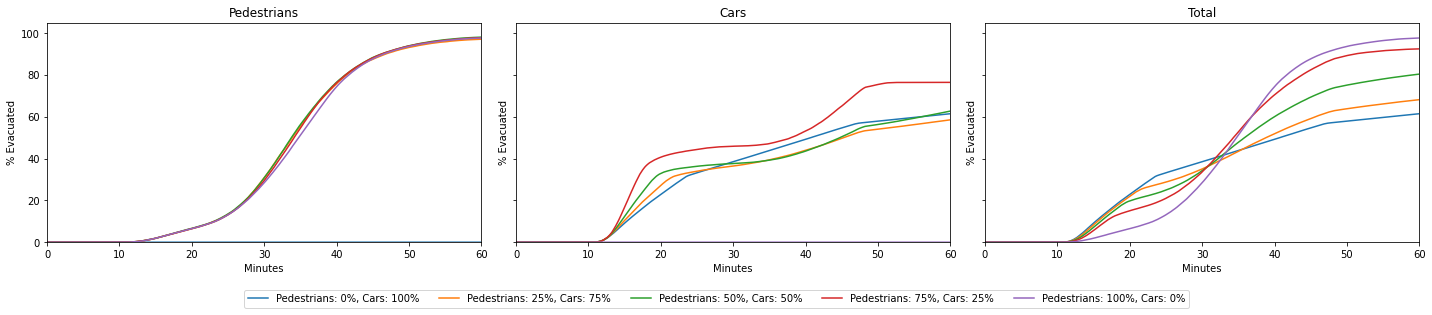
\includegraphics[width=\textwidth]{images/analisi/new-evacuated.png}
    \caption{}
    \label{fig:analisi-new-evacuated}
\end{figure}

\begin{figure}[ht]
    \centering
    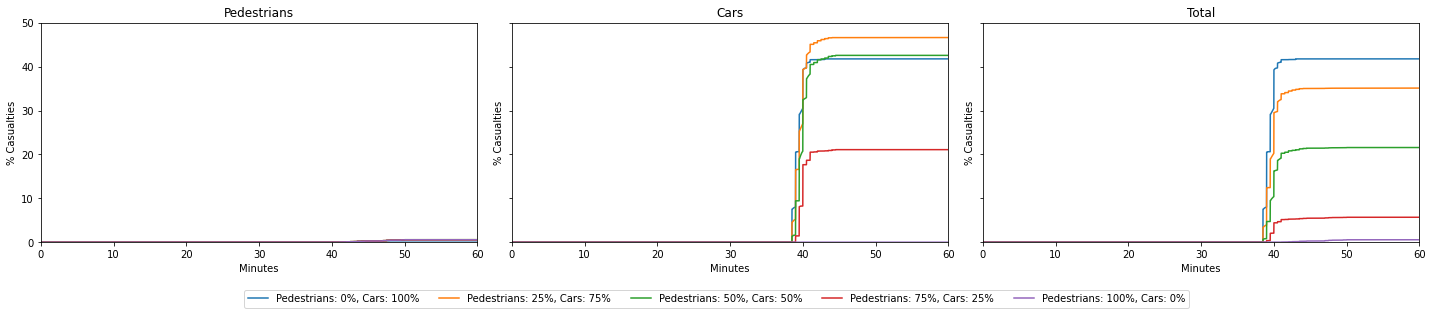
\includegraphics[width=\textwidth]{images/analisi/new-casualties.png}
    \caption{}
    \label{fig:analisi-new-casualties}
\end{figure}

\newpage
\begin{figure}[ht]
    \centering
    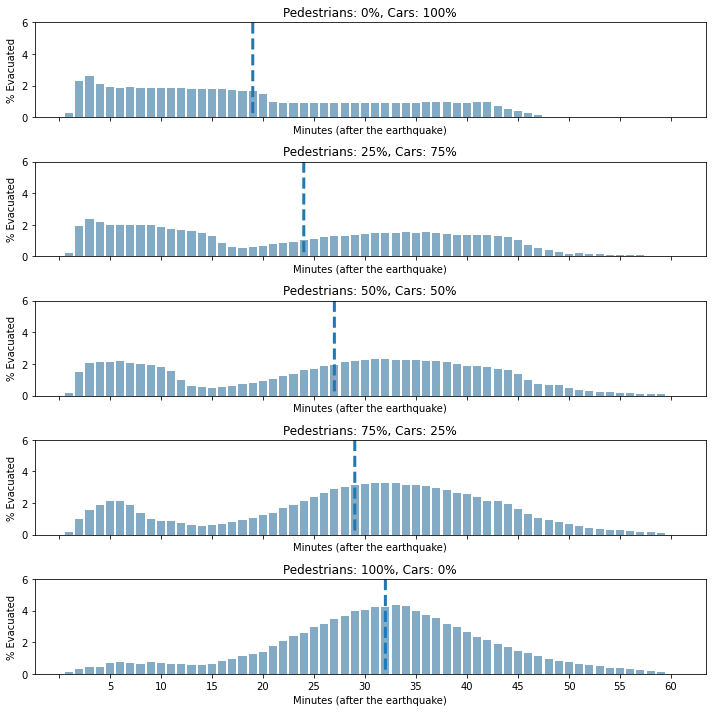
\includegraphics[width=\textwidth]{images/analisi/new-evtimes.png}
    \caption{}
    \label{fig:analisi-new-evtimes}
\end{figure}

\newpage

\subsection*{Comparazione Modello Base con Estensioni}
In questa sottosezione verrano comparati il modello base con il modello esteso analizzando,
le percentuali di evacuati e di morti nel tempo al variare del numero di auto e pedoni per poi passare a comparazioni spaziali,
in particolare mostrando l´efficienza delle intersezioni e l´effetto causato durante la simulazione.

Osservando \label{fig:analisi-comparison-total-ec} è possibile comparare le percentuali di evacuati e morti a diversi split tra i due modelli.
In generale il modello esteso presenta un numero minore di evacuati ed un numero maggiore di morti, con un andamento peggiorativo all´aumentare del numero di auto
gli unici casi in cui il modello esteso si avvicina ai risultati del modello base sono il caso con solo pedoni ed il caso 75\%-25\%.

\begin{figure}
    \centering
    \begin{subfigure}{0.475\textwidth}
        \centering
        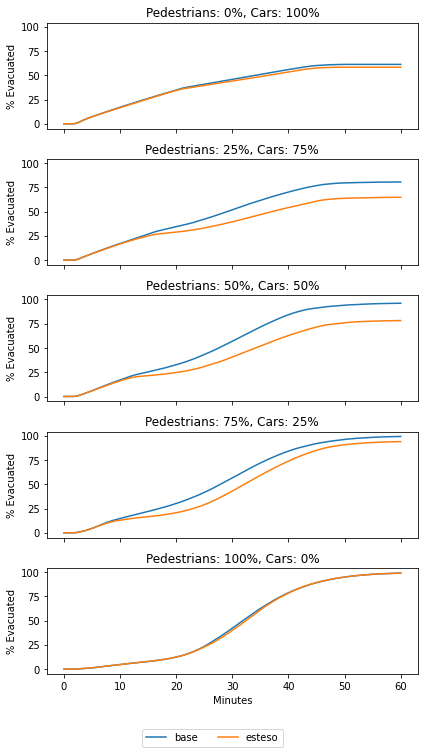
\includegraphics[width=\textwidth]{images/analisi/comparison-total-evacuated.png}
    \end{subfigure}
    \hfill
    \begin{subfigure}{0.475\textwidth}
        \centering
        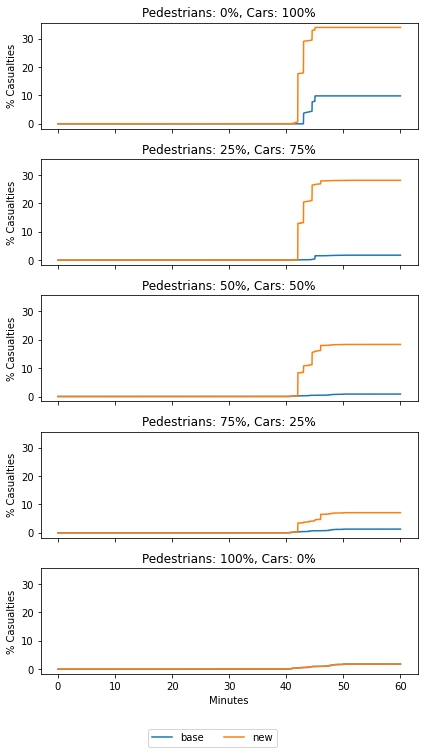
\includegraphics[width=\textwidth]{images/analisi/comparison-total-casualties.png}
    \end{subfigure}
    \caption{(a) comparazione \% evacuati tra modello base e modello esteso, (b) comparazione \% morti tra modello base e modello esteso}
    \label{fig:analisi-comparison-total-ec}
\end{figure}

Come già detto in precedenza le distribuzioni di percentuale di evacuati nel tempo \ref*{fig:analisi-comparison-evtimes} del modello base e del modello esteso 
presentano un andamento simile con un aumento del tempo medio di evacuazione.

\begin{figure}
    \centering
    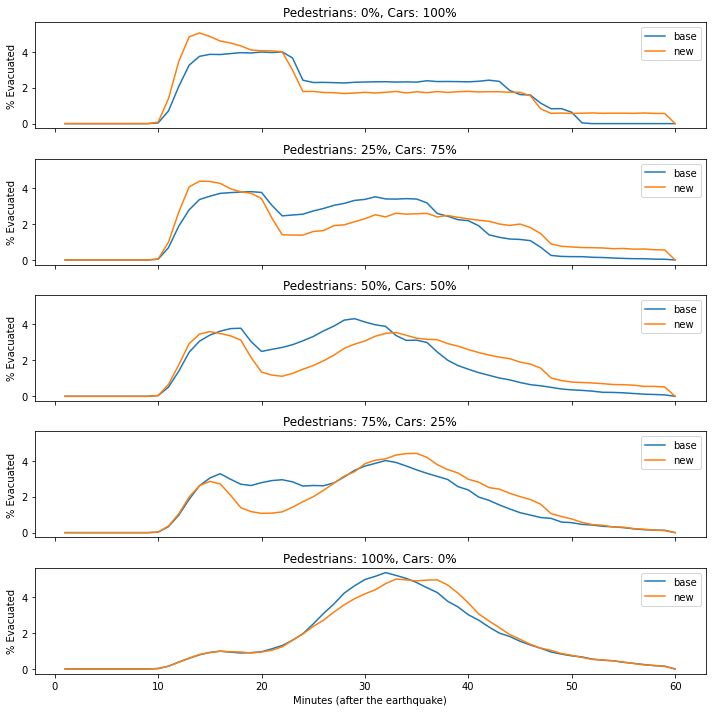
\includegraphics[width=\textwidth]{images/analisi/comparison-evtimes.png}
    \caption{}
    \label{fig:analisi-comparison-evtimes}
\end{figure}


Un´ulteriore comparazione è stata effettuata sui tempi di evacuazione al variare del numero di auto e pedoni
come si può vedere dal grafico \ref*{fig:analisi-comparison-evtimes2} il modello base presenta
un andamento decrescente del tempo medio richiesto per evacuare al diminuire delle auto, 
mentre il modello esteso ha sempre tempi maggiori del modello base ed i casi peggiori sono 25\% - 75\% e 50\% - 50\%.
I pedoni invece non presentano alcun cambiamento significativo ne al variare di split ne tra i due modelli con una media di circa 20min.

\ref*{fig:analisi-comparison-ev-times-map} mostra i tempi di evacuazione spazialmente in base al punto di partenza,
mediati tra tutte le possibili configurazioni di percentuali di auto e pedoni, si nota che in genrale chi parte sulla costa, la parte sinitra dell´immagine,
impiega più tempo di chi invece è più verso destra.
confrontando i casi (a) e (b) nessun cambiamente significativo viene introdotto dal modello esteso rispetto a quello base.
mentre per i casi (c) e (d) il modello esteso introduce dei rallentamenti soprattuto lungo la costa.

\begin{figure}
    \centering
    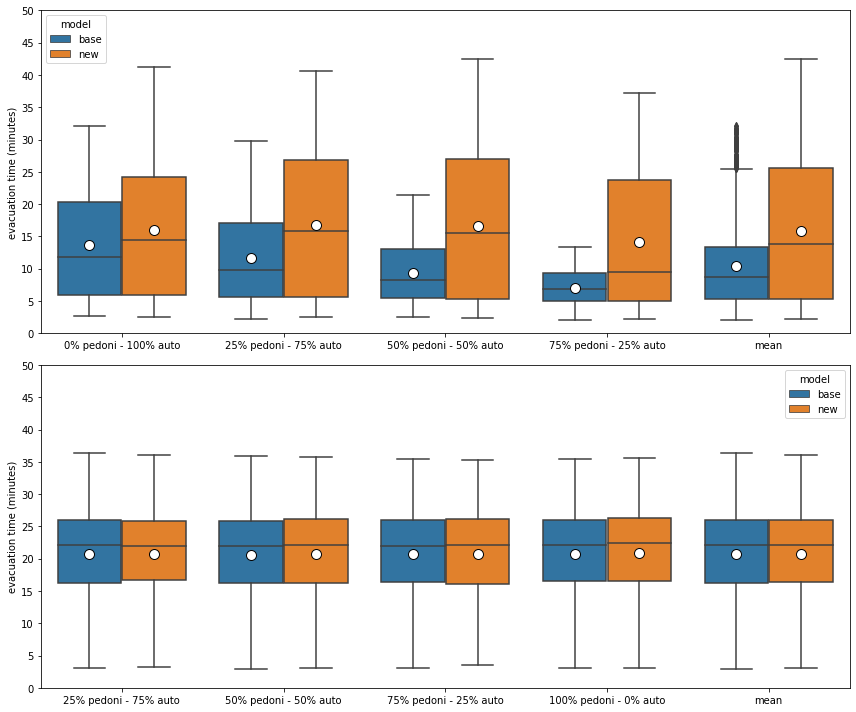
\includegraphics[width=\textwidth]{images/analisi/comparison-evtimes2.png}
    \caption{}
    \label{fig:analisi-comparison-evtimes2}
\end{figure}

\begin{figure}
    \centering
    \begin{subfigure}{0.475\textwidth}
        \centering
        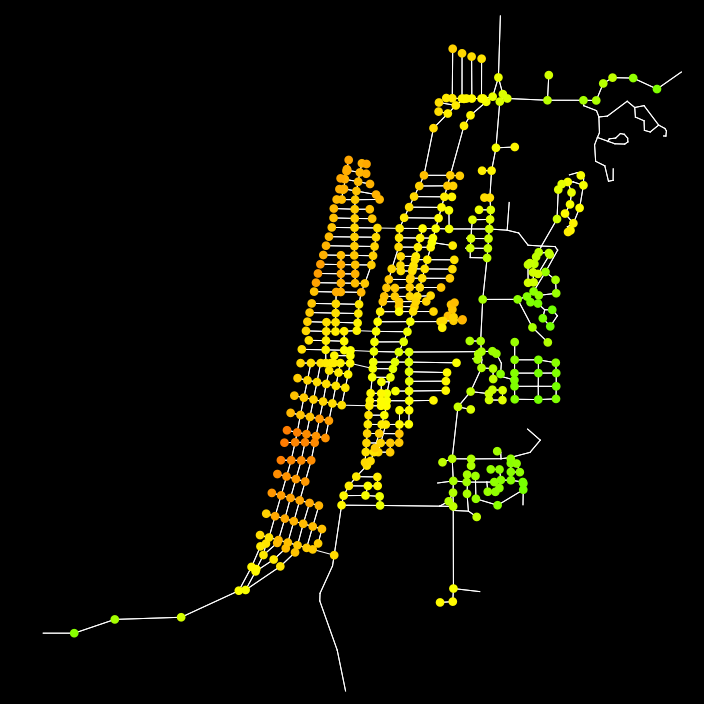
\includegraphics[width=\textwidth]{images/analisi/comparison-ev-times-map-base-car.png}
        \caption{base auto}
    \end{subfigure}
    \hfill
    \begin{subfigure}{0.475\textwidth}
        \centering
        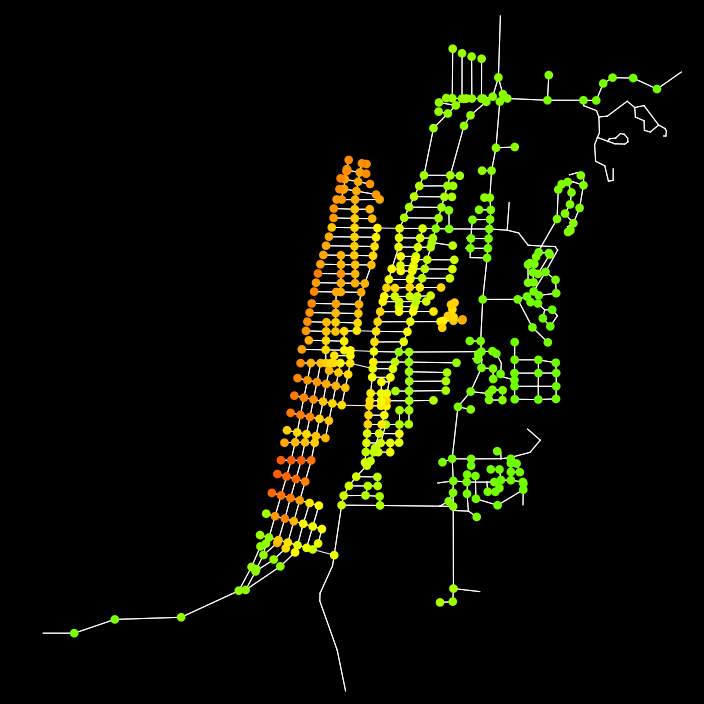
\includegraphics[width=\textwidth]{images/analisi/comparison-ev-times-map-new-car.png}
        \caption{new auto}
    \end{subfigure}
    \hfill
    \begin{subfigure}{0.475\textwidth}
        \centering
        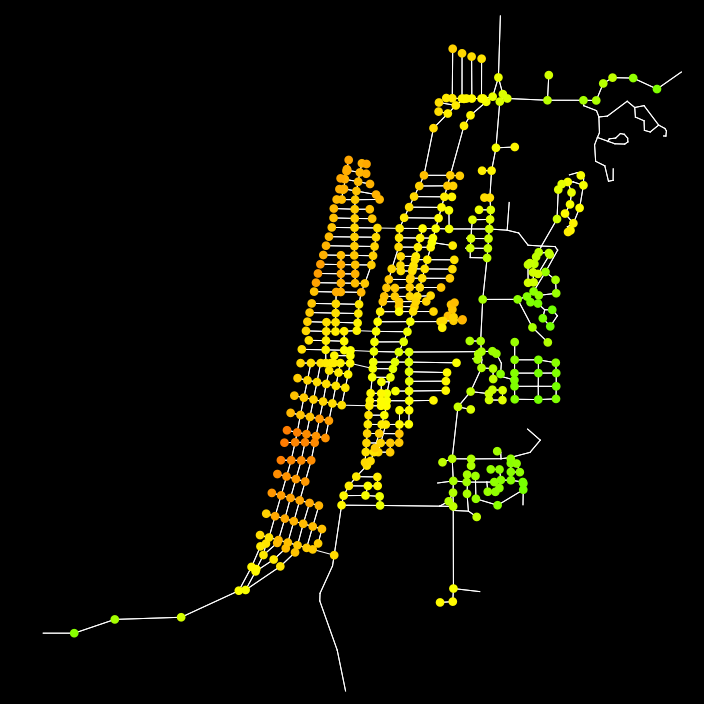
\includegraphics[width=\textwidth]{images/analisi/comparison-ev-times-map-base-ped.png}
        \caption{base pedoni}
    \end{subfigure}
    \hfill
    \begin{subfigure}{0.475\textwidth}
        \centering
        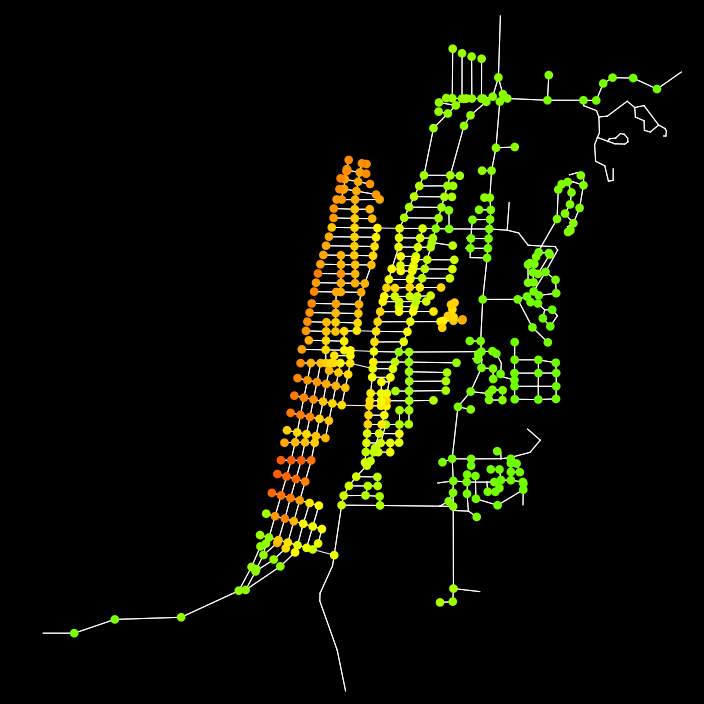
\includegraphics[width=\textwidth]{images/analisi/comparison-ev-times-map-new-ped.png}
        \caption{new pedoni}
    \end{subfigure}
    \caption{comparazione tempi di evacuazione rappresentati in base al punto di partenza dell´evacuazione}
    \label{fig:analisi-comparison-ev-times-map}
\end{figure}

Per valutare l´effetto casusato dalla gestione delle intersezioni i link critici dei due modelli sono stati comparati,
essi sono identificati analizzando la percentuale di mortalità media nei link e poi sogliati.
Il seguenti grafico \ref{fig:analisi-comparison-critical-links1} mostra la percentuale di mortalità
media nei link al variare dello split per il modello base e quello esteso, per poi sogliare al 5\%
la media dei vari split.
Osservando sia (a) che (b) si notano molti picchi più bassi con meno auto ed meno picchi più alti
all´aumentare del numero di auto, in generale il modello esteso presenta un numero maggiore di picchi più alti. 
I link critici identificati vengono riportati nel grafico \ref*{fig:analisi-comparison-critical-links2}.

\begin{figure}
    \centering
    \begin{subfigure}{0.475\textwidth}
        \centering
        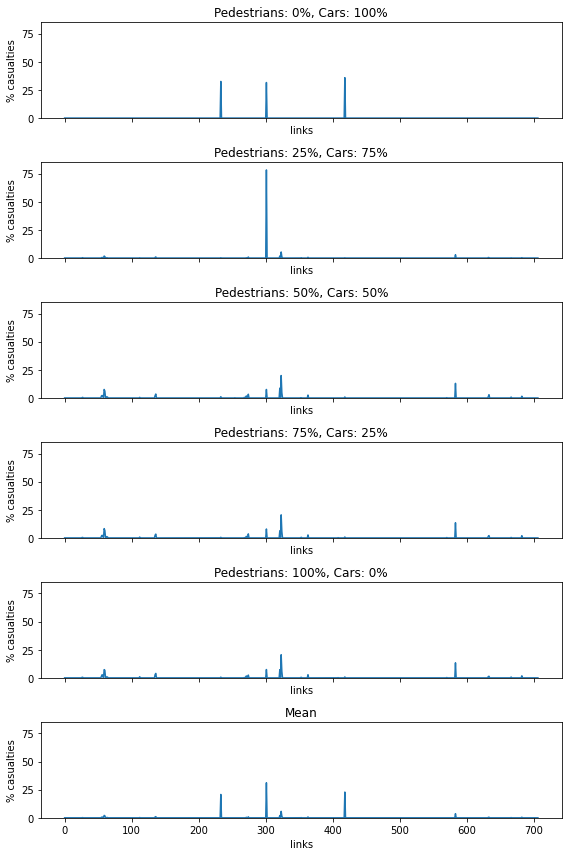
\includegraphics[width=\textwidth]{images/analisi/base_links_casualties.png}
        \caption{}
    \end{subfigure}
    \hfill
    \begin{subfigure}{0.475\textwidth}
        \centering
        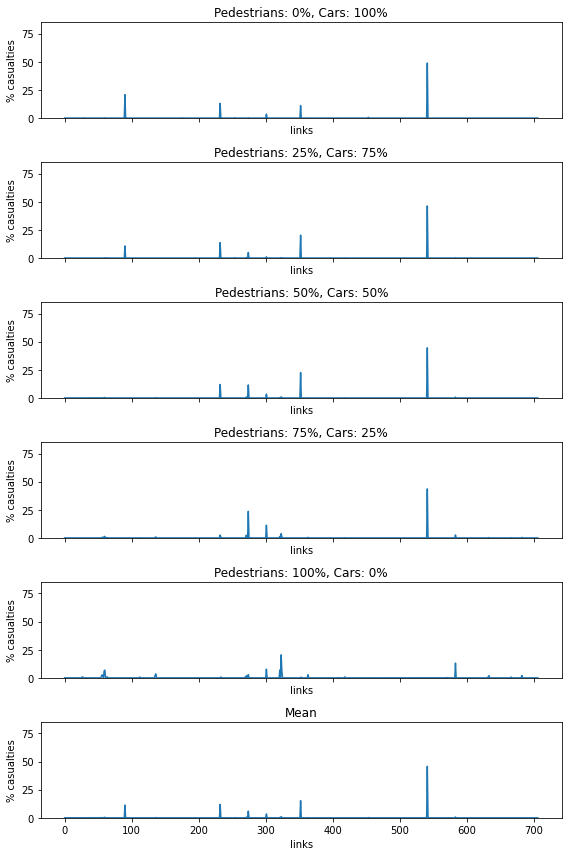
\includegraphics[width=\textwidth]{images/analisi/new_links_casualties.png}
        \caption{}
    \end{subfigure}
    \caption{}
    \label{fig:analisi-comparison-critical-links1}
\end{figure}

\begin{figure}
    \centering
    \begin{subfigure}{0.475\textwidth}
        \centering
        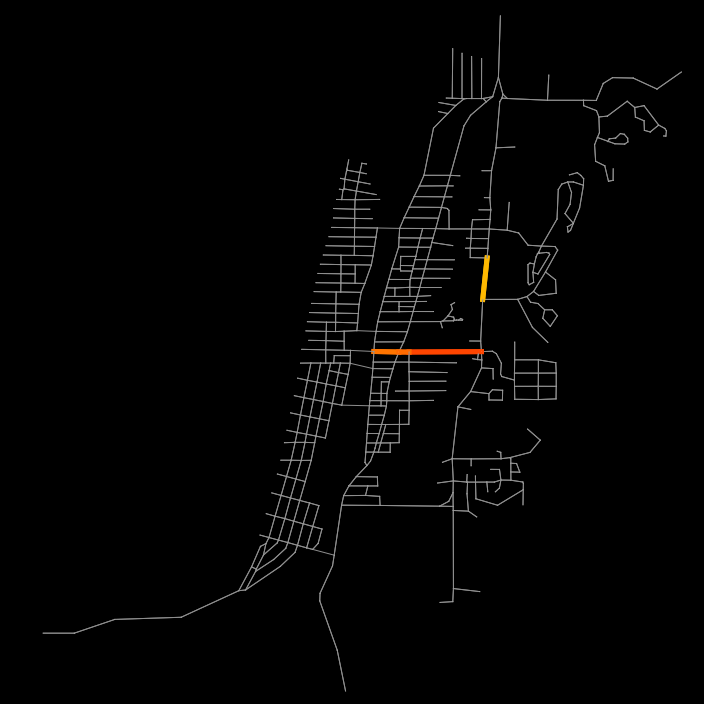
\includegraphics[width=\textwidth]{images/analisi/comparison-base-critical-links.png}
        \caption{}
    \end{subfigure}
    \hfill
    \begin{subfigure}{0.475\textwidth}
        \centering
        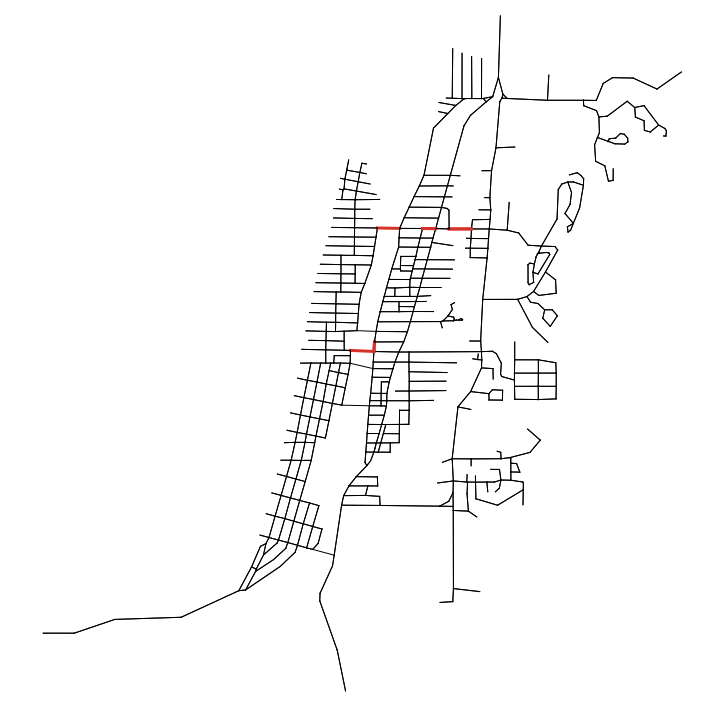
\includegraphics[width=\textwidth]{images/analisi/comparison-new-critical-links.png}
        \caption{}
    \end{subfigure}
    \caption{}
    \label{fig:analisi-comparison-critical-links2}
\end{figure}


\begin{figure}
    \centering
    \begin{subfigure}{0.99\textwidth}
        \centering
        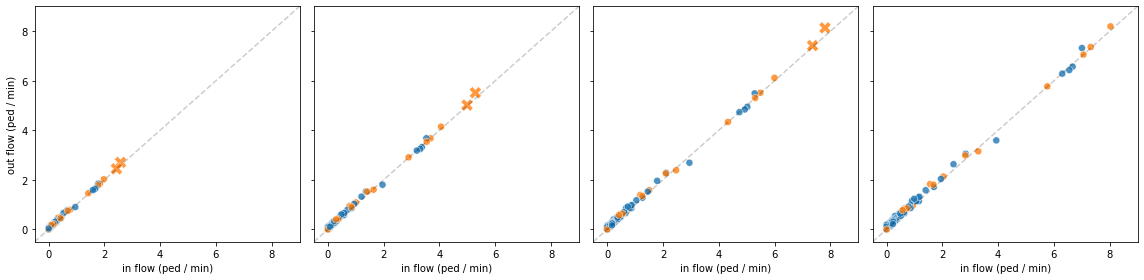
\includegraphics[width=\textwidth]{images/analisi/comparison-base-in-out-flow-ped.png}
        \caption{}
    \end{subfigure}
    \begin{subfigure}{0.99\textwidth}
        \centering
        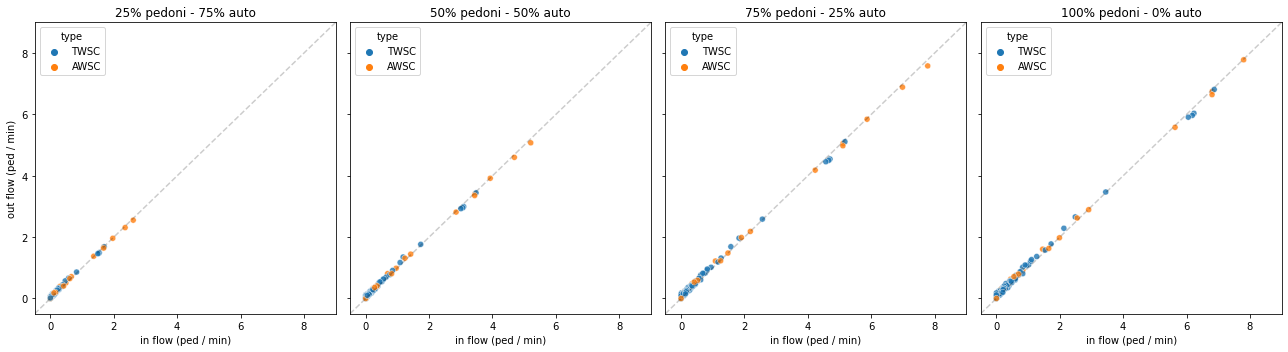
\includegraphics[width=\textwidth]{images/analisi/comparison-new-in-out-flow-ped.png}
        \caption{}
    \end{subfigure}
    \caption{}
    \label{fig:analisi-comparison-in-out-flow-ped}
\end{figure}

\begin{figure}
    \centering
    \begin{subfigure}{0.99\textwidth}
        \centering
        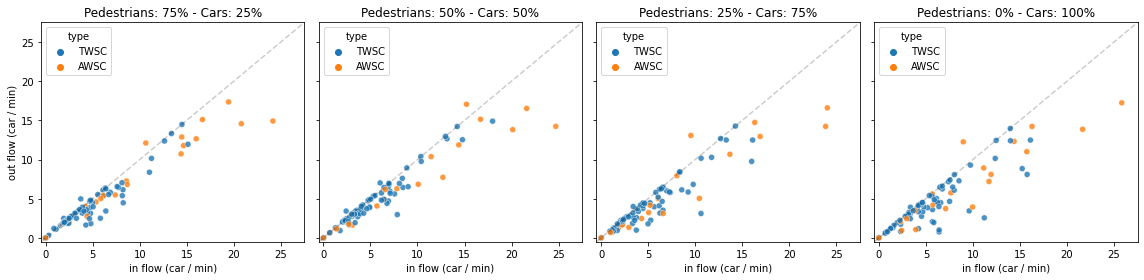
\includegraphics[width=\textwidth]{images/analisi/comparison-base-in-out-flow-car.png}
        \caption{}
    \end{subfigure}
    \begin{subfigure}{0.99\textwidth}
        \centering
        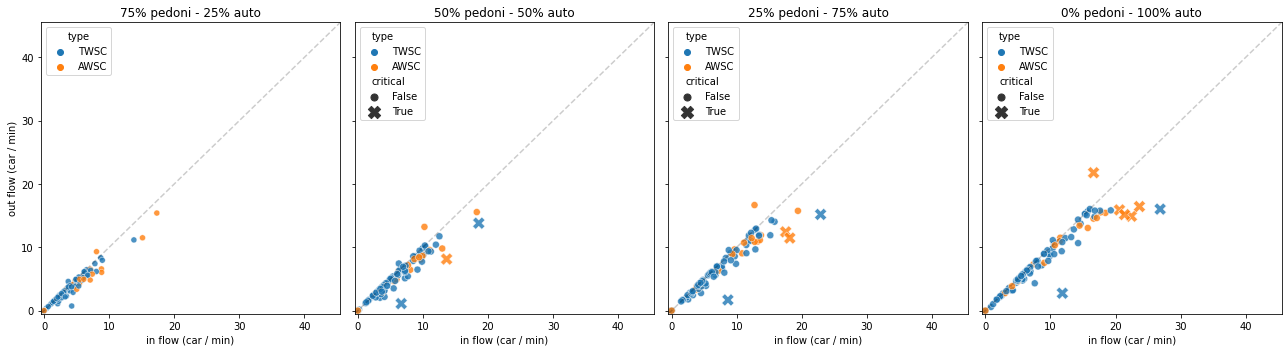
\includegraphics[width=\textwidth]{images/analisi/comparison-new-in-out-flow-car.png}
        \caption{}
    \end{subfigure}
    \caption{}
    \label{fig:analisi-comparison-in-out-flow-car}
\end{figure}

\begin{figure}
    \centering
    \begin{subfigure}{0.475\textwidth}
        \centering
        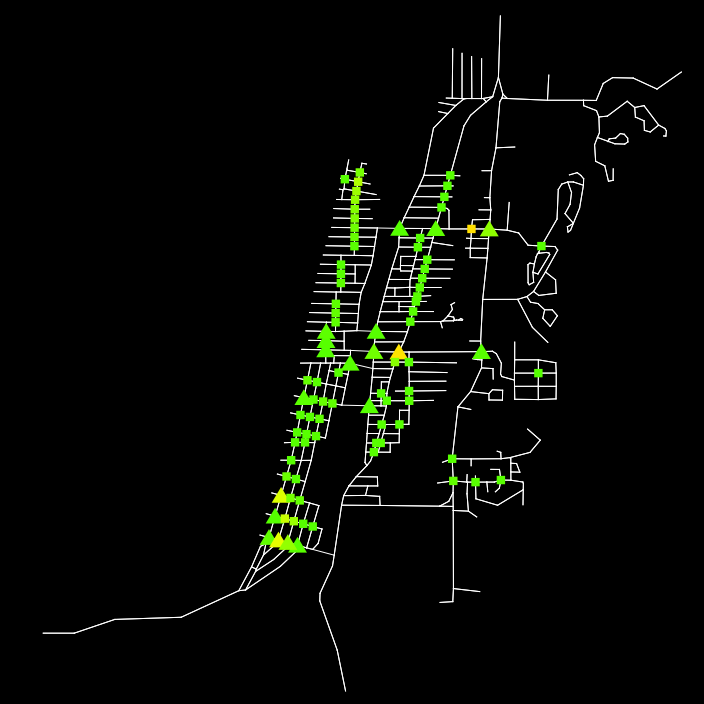
\includegraphics[width=\textwidth]{images/analisi/comparison-base-in-out-flow-75-25-car.png}
        \caption{75 pedoni 25 auto}
    \end{subfigure}
    \begin{subfigure}{0.475\textwidth}
        \centering
        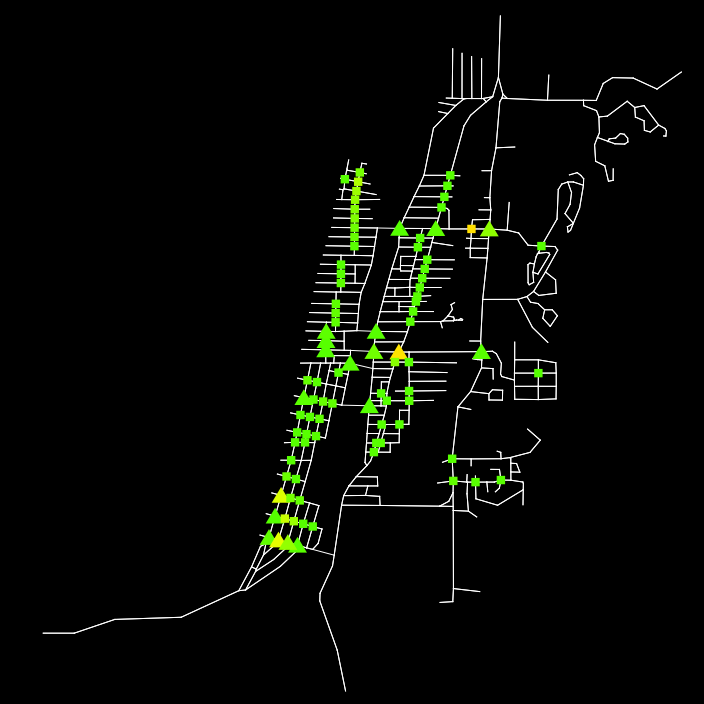
\includegraphics[width=\textwidth]{images/analisi/comparison-base-in-out-flow-50-50-car.png}
        \caption{50 pedoni 50 auto}
    \end{subfigure}
    \begin{subfigure}{0.475\textwidth}
        \centering
        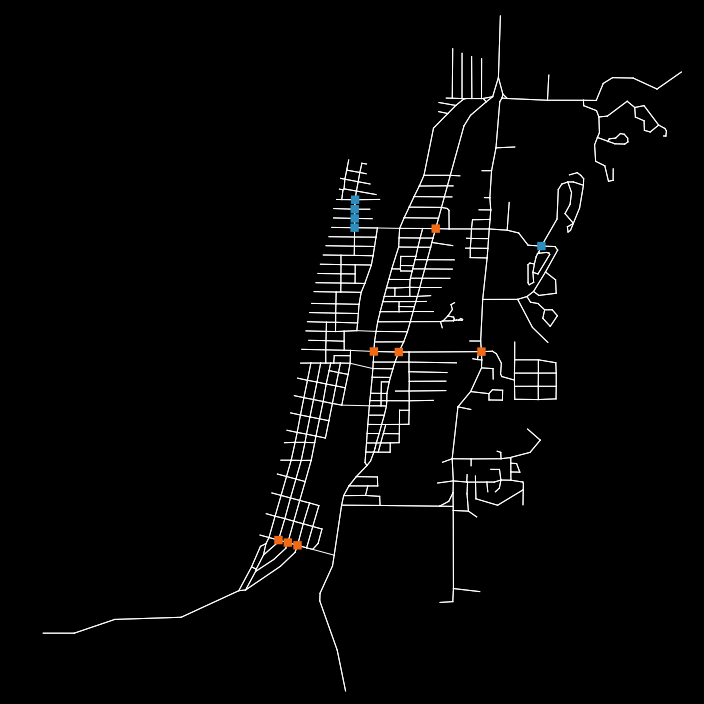
\includegraphics[width=\textwidth]{images/analisi/comparison-base-in-out-flow-25-75-car.png}
        \caption{25 pedoni 75 auto}
    \end{subfigure}
    \begin{subfigure}{0.475\textwidth}
        \centering
        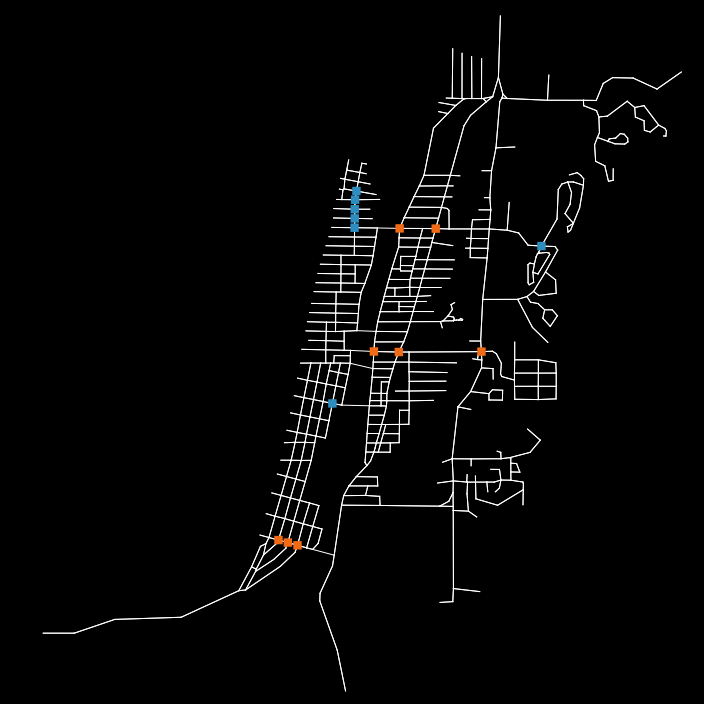
\includegraphics[width=\textwidth]{images/analisi/comparison-base-in-out-flow-0-100-car.png}
        \caption{0 pedoni 100 auto}
    \end{subfigure}
    \caption{}
    \label{fig:analisi-comparison-in-out-flow-map-base}
\end{figure}

\begin{figure}
    \centering
    \begin{subfigure}{0.475\textwidth}
        \centering
        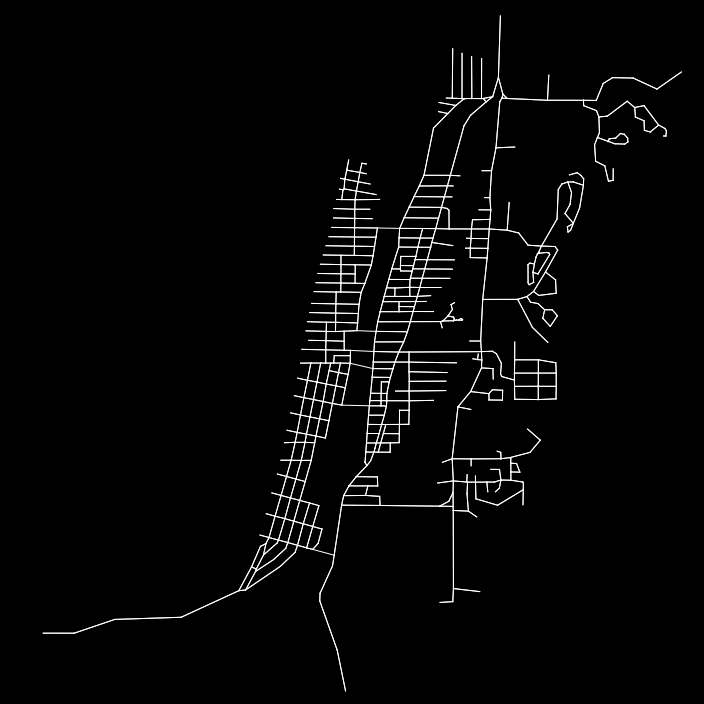
\includegraphics[width=\textwidth]{images/analisi/comparison-new-in-out-flow-75-25-car.png}
        \caption{75 pedoni 25 auto}
    \end{subfigure}
    \begin{subfigure}{0.475\textwidth}
        \centering
        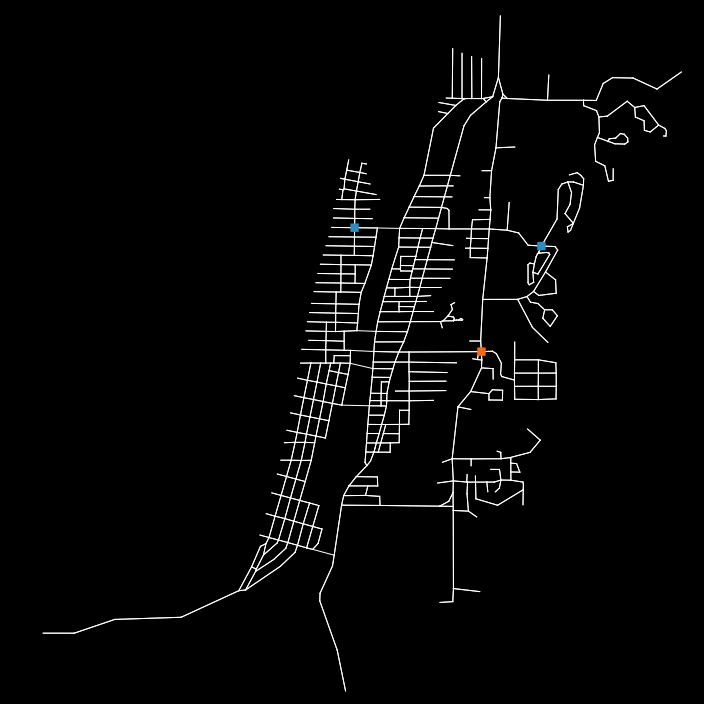
\includegraphics[width=\textwidth]{images/analisi/comparison-new-in-out-flow-50-50-car.png}
        \caption{50 pedoni 50 auto}
    \end{subfigure}
    \begin{subfigure}{0.475\textwidth}
        \centering
        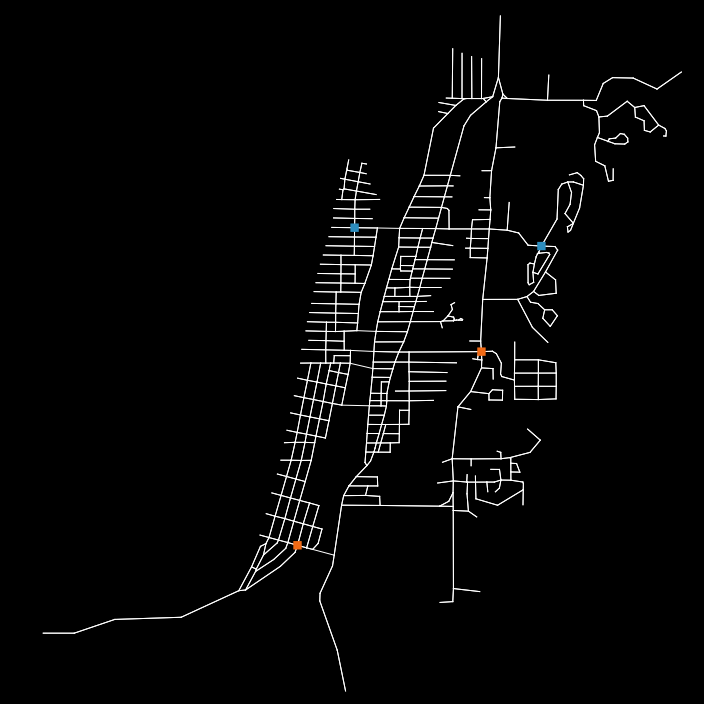
\includegraphics[width=\textwidth]{images/analisi/comparison-new-in-out-flow-25-75-car.png}
        \caption{25 pedoni 75 auto}
    \end{subfigure}
    \begin{subfigure}{0.475\textwidth}
        \centering
        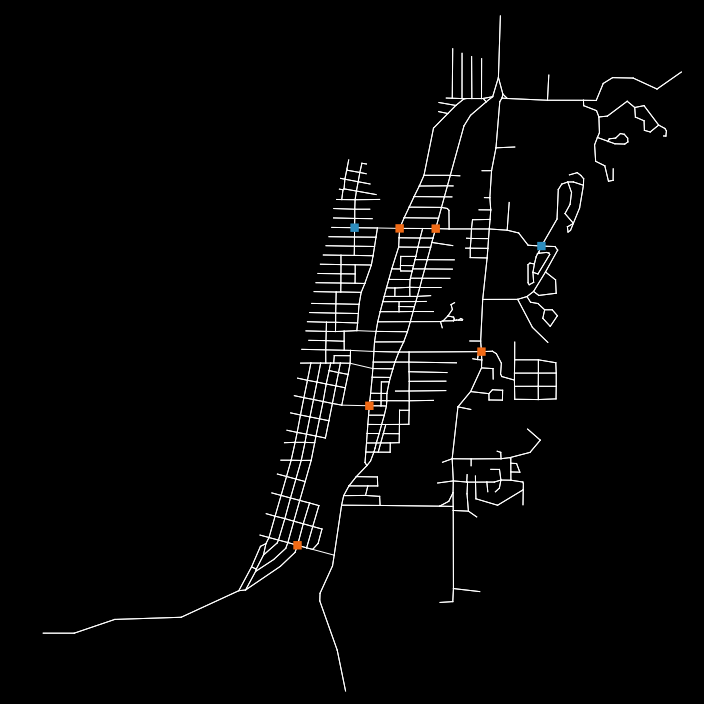
\includegraphics[width=\textwidth]{images/analisi/comparison-new-in-out-flow-0-100-car.png}
        \caption{0 pedoni 100 auto}
    \end{subfigure}
    \caption{}
    \label{fig:analisi-comparison-in-out-flow-map-new}
\end{figure}

Infine per il modello esteso vengono analizzati i tempi di attesa nelle intersezioni,
ovvero il tempo che passa da quando arriva all´incrocio ed aspetta
il via libera, differenziando tra i due tipi di incrocio AWSC e TWSC.
Come si pu`o vedere nella tabella \ref*{tab:analisi-car-delay} con un numero minore di auto le intersezioni AWSC 
in media hanno alti tempi di attesa mentre i TWSC hanno tempi bassi.
All´aumentare del numero di auto si abbassano in media i tempi di attesa negli AWSC e si alzano quelli dei TWSC.
In \ref*{fig:analisi-comparison-car-delay} vengno riportati i tempi di attesa nelle intersezioni spazialmente
dove i triangoli rappresentano gli AWSC mentre i quadrati i TWSC.

\begin{table}[ht]
    \centering
    \begin{tabular}{|c|c|c|c|c|c|}
    \hline
         & 75-25 & 50-50 & 25-75 & 0-100 & intersection \\ \hline
    mean & 34 s  & 32 s  & 29 s  & 24 s  & AWSC         \\ \hline
    max  & 267 s & 184 s & 202 s & 225 s & AWSC         \\ \hline
    mean & 8 s   & 13 s  & 18 s  & 31 s  & TWSC         \\ \hline
    max  & 142 s & 189 s & 237 s & 406 s & TWSC         \\ \hline
    \end{tabular}
    \caption{tempo di attesa per le auto alle intersezioni al variare dello split}
    \label{tab:analisi-car-delay}
\end{table}

\begin{figure}
    \centering
    \begin{subfigure}{0.475\textwidth}
        \centering
        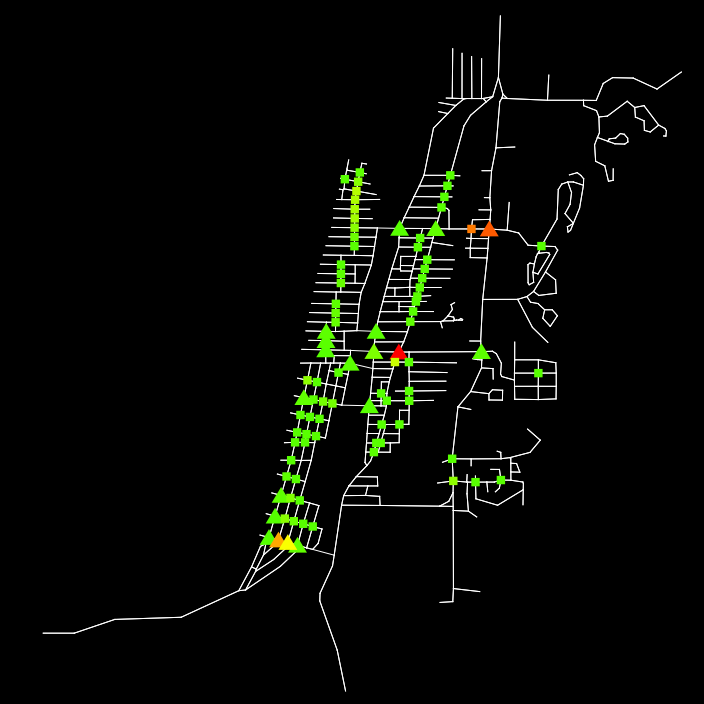
\includegraphics[width=\textwidth]{images/analisi/comparison-car-delay-75-25.png}
        \caption{75 pedoni 25 auto}
    \end{subfigure}
    \begin{subfigure}{0.475\textwidth}
        \centering
        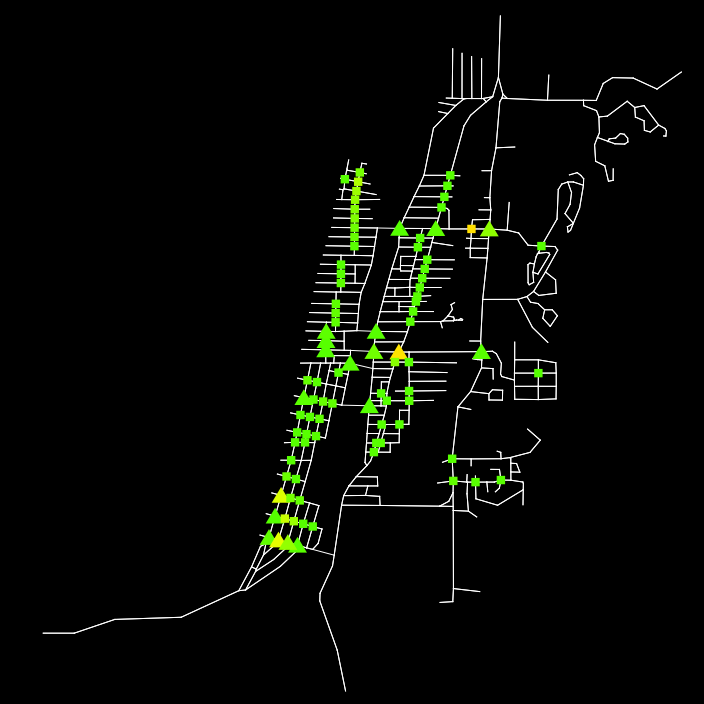
\includegraphics[width=\textwidth]{images/analisi/comparison-car-delay-50-50.png}
        \caption{50 pedoni 50 auto}
    \end{subfigure}

    \begin{subfigure}{0.475\textwidth}
        \centering
        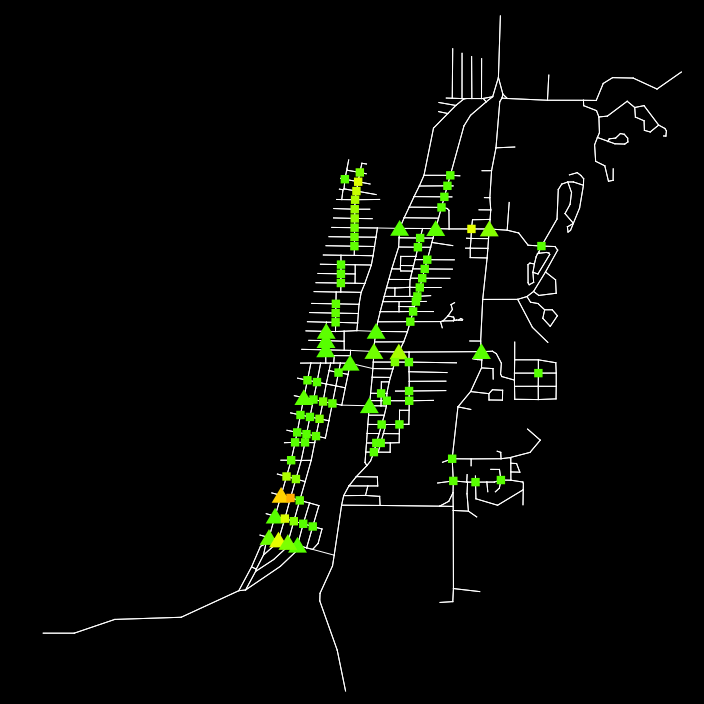
\includegraphics[width=\textwidth]{images/analisi/comparison-car-delay-25-75.png}
        \caption{25 pedoni 75 auto}
    \end{subfigure}
    \begin{subfigure}{0.475\textwidth}
        \centering
        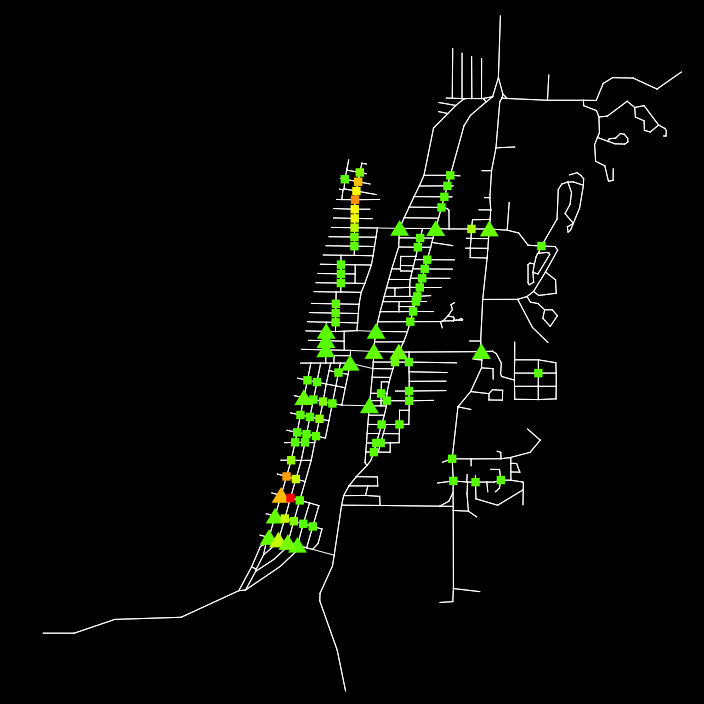
\includegraphics[width=\textwidth]{images/analisi/comparison-car-delay-0-100.png}
        \caption{0 pedoni 100 auto}
    \end{subfigure}
    \caption{}
    \label{fig:analisi-comparison-car-delay}
\end{figure}

\subsection*{Comparazione Modello Base con Modello Wang 2021}
